%\documentclass[authoryear,round]{tufte-book}
\documentclass[a4paper,10pt]{article}
\usepackage[T1]{fontenc}
\usepackage[utf8]{inputenc}
\usepackage{amsmath}
\usepackage{amssymb}
\usepackage{graphicx}
\usepackage{fullpage}
\usepackage{color}
\usepackage{natbib}
\usepackage{mathrsfs}
\usepackage{array}
\newcommand{\head}[2]{\multicolumn{1}{>{\centering\arraybackslash}p{#1}}{#2}}
%\usepackage{sidecap}
\usepackage[capbesideposition={top,right},facing=yes,capbesidesep=quad]{floatrow}
\usepackage[hypertexnames=false]{hyperref}
\hypersetup{colorlinks=true, urlcolor=blue, citecolor=black, linkcolor=black}
%\usepackage{lineno}
%\usepackage{lscape}
%\usepackage{multirow}

\newcommand{\var}{\mathop{\mbox{Var}}}
\newcommand{\cov}{\mathop{\mbox{Cov}}}
\newcommand{\gc}[1]{{\it \color{red} (#1)} }
\newcommand{\jb}[1]{{\it\color{blue} (#1)} }
\def\citeapos#1{\citeauthor{#1}'s (\citeyear{#1})}
%\newcommand{\Rho}{\mathrm{P}}

%opening
\title{Theory of Sweeps from Standing Variation}
\author{
Jeremy J. Berg$^{1,2,3}$ and Graham Coop$^{1,2,3}$ \\
$^1$ Graduate Group in Population Biology, University of California, Davis. \\
$^2$ Center for Population Biology, University of California, Davis.\\
$^3$ Department of Evolution and Ecology, University of California, Davis\\
\small To whom correspondence should be addressed: \texttt{jjberg@ucdavis.edu, gmcoop@ucdavis.edu}\\
}

\date{}

\begin{document}

%\linenumbers
\maketitle

\begin{abstract}
\end{abstract}

%%%%%%%%%%%%%%%%%%%%%%%%%%%
\section{Introduction}



%%%%%%%%%%%%%%%%%%%%%%%%%%%
\section{Results}
\jb{thinking perhaps we should motivate our whole framework with a fair bit of verbal description before we delve into any math. Ideas here are reletively straightforward, but a fair bit of ``scene setting'' to do first}

The key insight for this paper is that the recombination events that occur during the period when an allele is neutral or balanced prior to a sweep can be treated like mutations, and thus under the assumption of constant population size, we can use the Ewens Sampling Formula to calculate expectations for a variety of quantities of interest in the region surrounding the selected site.

Consider a neutral locus partially linked (with recombination rate $r$) to a second locus where an allele arises, and is initially either neutral, or balanced at a low frequency, but eventually becomes beneficial (due to a change in environment). Our aim is to describe some features of the genealogy at the selected site at at adjacent neutral sites, how these features effect a number of population genetic summary statistics, and to explore the extent to which they can be used to say anything meaningful about sites where sweeps from standing variation may have occurred. 

\begin{figure}
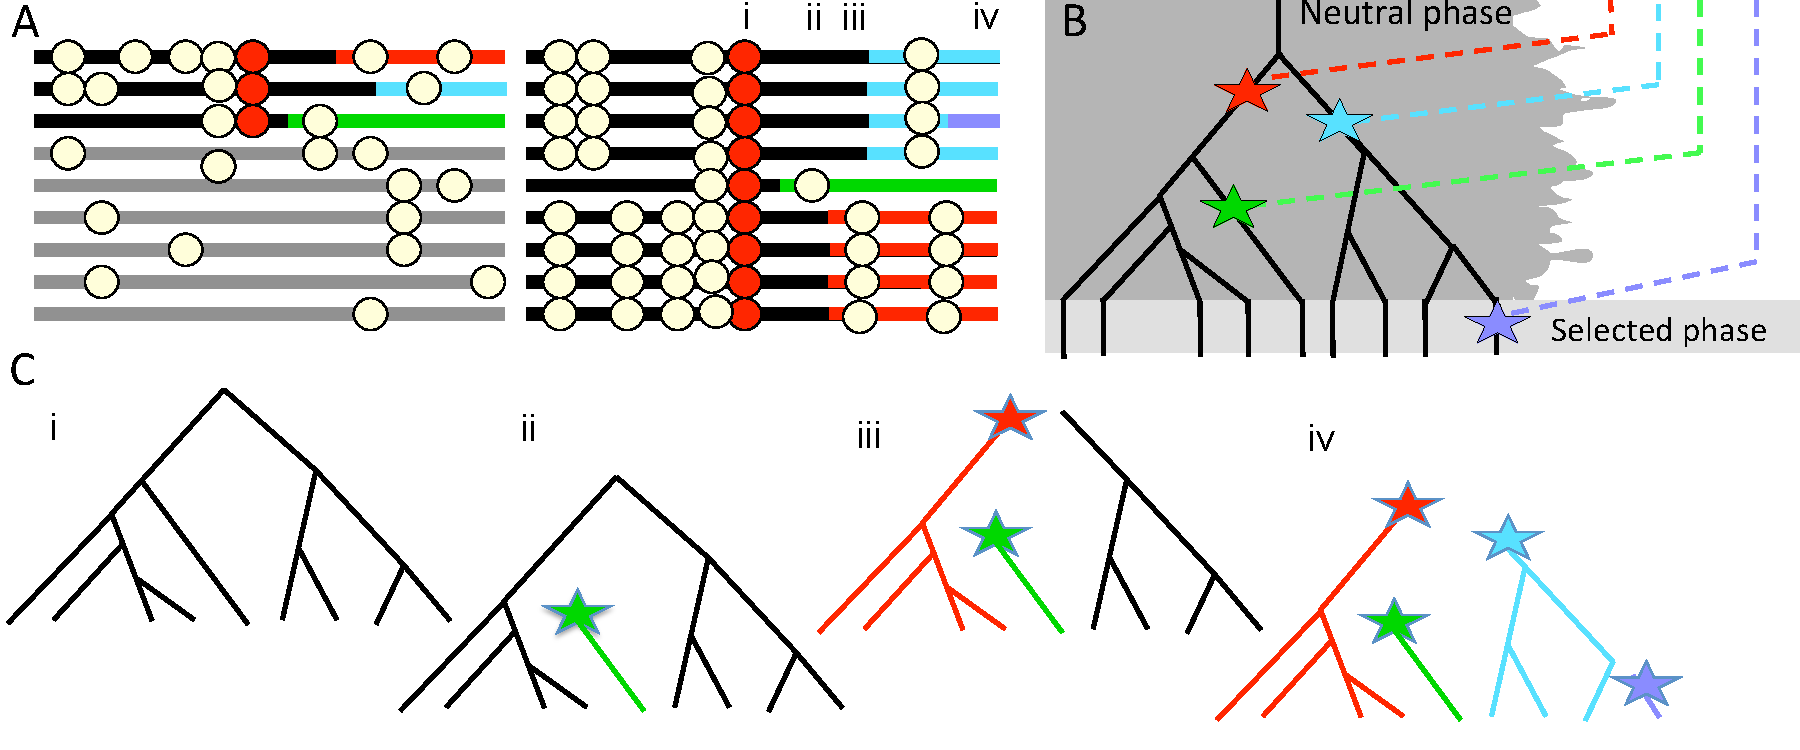
\includegraphics[width = 0.8
          \textwidth]{Paper_Figures/Cartoon_of_soft_sweeps.pdf}
\end{figure}

\subsubsection{Neutral phase} \gc{not clear that neutral is a good term}
Imagine that we sample $k$ neutral alleles (lineages) from the population in the present day. 
We will assume that the selected phase of the trajectory occurs rapidly so there is no timefor coalescence to occur in the selected phase. So at the start of the neutral phase we have k lineages and the frequency of the selected allele is $f$ on the population.

We will argue that the majority of information about patterns of diversity surrounding a sweep from standing variation can be understood by understanding the genealogy at the selected site,
and where recombinations fall on this genealogy as we move away from the selected sites. 

If our allele was held fixed at low frequency $f$ over a long time period our genealogy at the selected site would simply be a coalescent where any pair of lineages at rate $ {k \choose 2}/(2 N f)$ (assuming that $f \gg 1/(2N)$ so that the standard coalescent assumptions hold). Such a fixed frequency could result from a beneficial allele that was balanced at low frequency, by strong constant selection. If instead of being held fixed at a frequency $f$ our allele was allowed to drift neutrally this constant pairwise coalescent rate would no long be appropriate as the frequency could have changed to $f^{\prime} \neq f$, and so now our instantaneous rate of coalescence would be  $1/(2Nf^{\prime})$. 

A number of researchers have studied the behavior of the coalescent within a neutral mutant subclass \citep{XXXX}, either conditional on the frequency of the allele in a sample or in the population.. \cite{XXX} has shown that the expected coalescent time is  $2 N f/ {k \choose 2}$ in the absence of other information, e.g. as to whether the allele is ancestral or derived or other information about the frequency of the allele in the past. However, the distribution of coalescence times is no longer exponential, and the successive coalscent times are not independent \cite{} as the time it takes a pair of lineages to coalescence contains information about the current frequency of the allele and thus about susequent coalescent events. Furthermore, when the allele is known to be derived the coalescent times have a more complicated expectation, as the allele is in expectation decreasing in frequency backward in time due to the conditioning on loss \citep{}.

Despite these complications we have found assuming that lineages to coalesce at a rate $ {k \choose 2}/(2 N f)$ and that coalescent time intervals are independent, i.e. that the allele frequency does not drift from $f$, is not a bad approximation when $f \ll 1$ regardless of whether the allele is ancestral or derived. In Supp. Figures XXX-XXX we show some comparisons of the coalescent process inbedded in a drifting allele frequency and this approximation. 

The main reason for using this approximation is that is gives us a simple well understood characture of the true process that describes the genealogy at the selected site reasonably accurately. We can use this to understand patterns of recombination as we move away from the selected site. We will again rely on the assumption that $f \ll 1$, and assume that any lineage that recombines out of the background of our beneficial allele will not recombine back into the background. As further consequence of $f \ll 1$ the coalescent times in our beneficial allele class (on a time-scale $\propto 2Nf$) will be short compared to those in the other allelic class (on a time-scale $\propto 2Nf(1-f)$). As such, we will ignore coalescent events in the other allelic class. Under these two assumptions as we move away from the selected site, recombinations are events on our genealogy at the selected site that peels lineages out from the selected class allowing them to coalescence on much longer time scales. In Figure \ref{cartoon_fig_1}B we show the coalescent genealogy at the selected site, and show recombination events out of the benefical allele class imposed on the genealogy (these events are colored to correspond to the events on the haplotypes in Figure \ref{cartoon_fig_1}A). In 
Figure \ref{cartoon_fig_1}C we show the genealogy at various points along the sequence shown in Figure \ref{cartoon_fig_1}A, between recombination events. 

Assuming that the frequency of the allele remains fixed at $f$, at a distance $r$ away from the selected site a lineage recombines out of the selected class at rate $r(1-f)$ \gc{Still wonder if we should make this just $r$, as we are assuming $(1-f) \approx 1$ elsewhere}. As coalescent occurs at a rate ${k \choose 2}/(2Nf)$, we can rescale time in units of $2Nf$ so that coalescence happens at a rate ${k \choose 2}$, and recombination events out of the selected class happen at rate $2Nrf(1-f)$. 

If we are interested in the number and size of different recombinant clades at a given distance from the selected site (colored clades in Figure \ref{cartoon_fig_1}B \& C)  this a direct analogy of the infinitely-many allele model \citep{}. In the infinite alleles model, every mutation event creates a new allele, while in our process every recombination event creates a new recombinant lineage (an potentially a distinct haplotype, depending on the configuration of mutations). Under the infinitely many alleles model, sample configurations can be found by simulating the coalescent and assigning current day alleles is found by lineages back through time to the lowest mutation on the genealogy (see Figure \ref{cartoon_fig_1}B). Equivalently we can simulate a sample under the infinitely-many allele model by simulating the mutational process and coalescent process simulatenously, running the process back coalescing lineages and stopping following lineages (`kill' them) when a mutation occurs on them (see Figure \ref{cartoon_fig_1}C). 

Given this nice direct analogy under our set of approximations the number and frequency of the various recombinant lineage classes at a given distance from the selected site can be found using the Ewens' Sampling Formula \citep[ESF][]{}.The population-scaled mutation rate in the infinitely-many alleles model ($\theta/2=4N\mu$), in our model, is replaced by the rate of recombination out of the selected class ($R_{f}/2=4Nrf(1-f)$). If $n$ lineages sampled in the present day fail to recombine off of the selected background during the course of the sweep, then the probability that these $n$ lineages coalesce into a set of $k$ recombinant lineages is 
\begin{equation}
p_{ESF}(k | R_f,n)  = S(n,k) \frac{R_f^i}{ \prod_{j=1}^{i-1} (R_f +j) }  \label{ESF1}
\end{equation}
where $S(n,k)$ is a Stirling number of the first kind
\begin{equation}
S(n,k) = \textrm{StirlingStirlingStirling}
\end{equation}
These recombinant lineages partition our sample up between themselves, so that each of these lineages have a number descendents in our present sample$\{n_1,n_2,\dots,n_k\}$, where $\sum_1^k n_i =n$. Conditional on $k$ the probability of a smaple configuration is
\begin{equation}
p(\{n_1,n_2,\dots,n_k\} \mid k,n) = \frac{n!}{k! n_1\cdots n_k S(n,k)}  \label{ESF2}
\end{equation}
Note this does not depend on $R_f$, which gives the classic result that the number of alleles is sufficient statistic for $R_f$ (i.e. the partition is not needed to estimate $R_f$). Note also that this is a slightly different form to that usually used for the ESF, usually the sample configuration is expressed as a frequency spectrum where we count up the number of alleles present once, twice, etc in our sample.

\begin{figure}
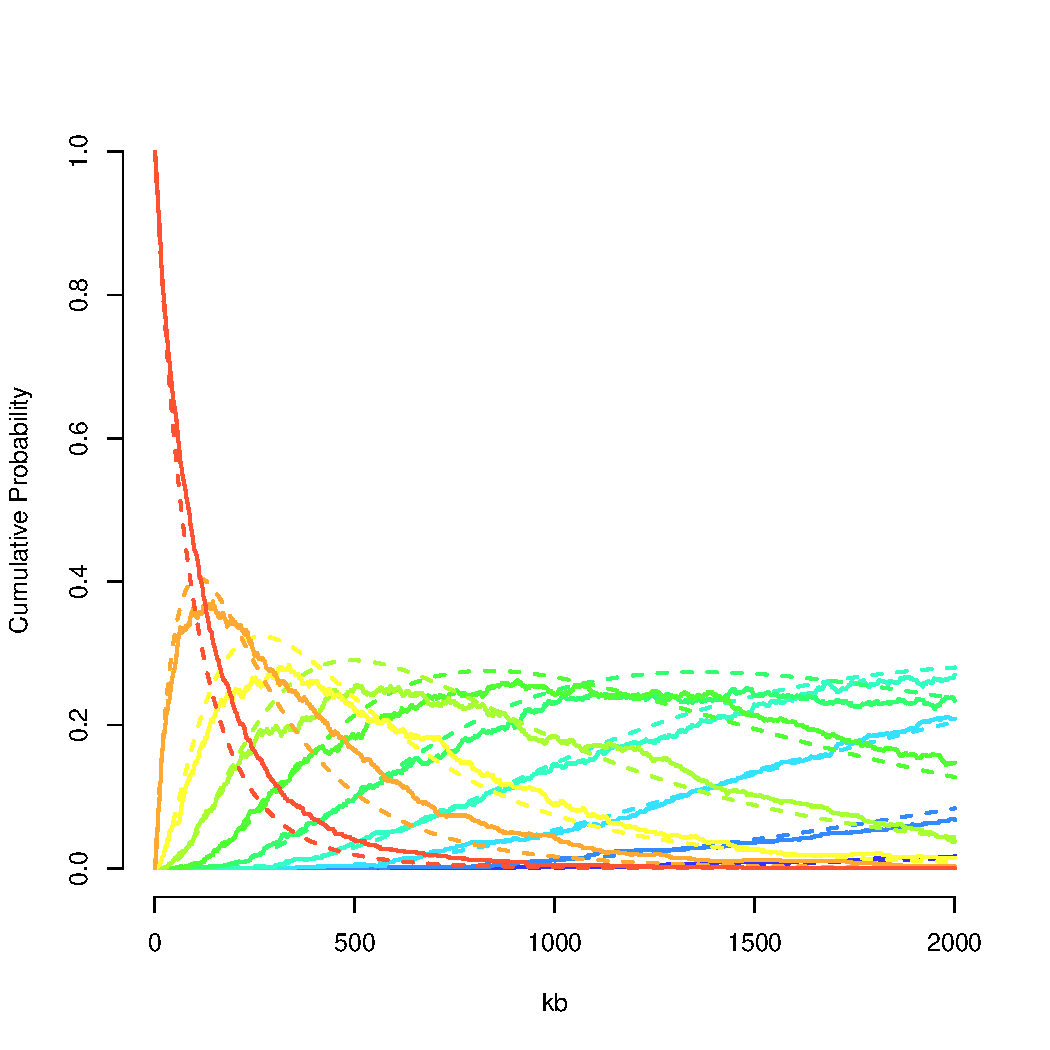
\includegraphics[width = 0.8
          \textwidth]{Paper_Figures/Ewens_vs_Jeremy.pdf}
\end{figure}

%and that the number of coalescent families with $1,2,\dots,n$ lineages is given by the partition
%  $\{n_1,n_2,\dots,n_k\}$ is 
% \begin{equation}
% P\left(k,n_1,n_2,\dots,n_n| R_f,n \right) =\frac{R_f^i}{ \prod_{j=1}^{i-1} (R_f +j) } \prod_{j=1}^n\frac{1}{j^{n_j}n_j!} \label{ESF}
% \end{equation}
% The probability of there being $k$ alleles (recombinant lineages) in our sample of $n$

\subsubsection{Selected phase}
Assume that we are at a neutral site a genetic distance $r$ away from the selected site. 
If we let $X\left(t\right)$ be the frequency of the selected allele at time $t$ in the past, the probability that a single lineage fails to recombine off in generation $t$ is $1-r\left(1-X(t)\right)$. The probability that a single lineage manages to recombine off the selected background at any point during the course of the sweep is given by 
\begin{equation}
P_{NR} \prod_{t=0}^{\tau} 1-r\left(1-X(t)\right)  \approx \exp \left(-r \int_0^{\tau}(1-X\left(t\right))\mathrm{d} t\left(t\right) \right)
\end{equation}
for $r \ll 1$. We set  $\mathcal{T}_{\left(s,f\right)} = \int_0^{\tau}(1-X\left(t\right))\mathrm{d}t$, so that the probability that a lineage manages to recombine off the selected background during the course of the sweep is $e^{-r\mathcal{T}_{\left(s,f\right)}}$. If our selected allele has an additive avantage in terms of relative fitness of $s/2$ in heterozygotes and $s$ in homozygotes, then our allele's deterministic trajectory through the population is logistic and $\mathcal{T}_{\left(s,f\right)} =???$

We assume that the sweep occurs fast enough that the probability of coalescence during the sweep is essentially zero. Therefore, each lineage makes an independent choice of whether it recombines out of the sweep, so that the probability that $i$ out of $k$ lineages fail to escape off the sweep background is
\begin{equation}
P_{NR}(i;k) = {k \choose i} P_{NR}^{i} (1-P_{NR})^{k-i}.
\end{equation}
This binomial approximation has been made by a number of authors in the context of hard sweeps \citep{Barton}, and more accurate approximations have been developed \citep{}. However, as long as the population is large, the sample is not too large,  $\tau$ is not too long, and $f$ not too small (e.g. $\tau {k \choose 2}/(2Nf)<<1$) then this approximation should be adequet. The other more accurate forms could be incorporated into our framework, but we stick with this simple form for the sake of clarity of presentation.

At a given distance away from the selected site every one of the lineages that recombines out of the selected class will be a singleton, and the remaining lineages will be partitioned according to the Ewens' Sampling formula.  


\subsubsection{Patterns of neutral diversity surrounding standing sweeps}
Given this approximate model of the coalescent with a sweep from standing variation we can now calculate basic summaries of variation in the region surrounding the sweep. We will assume that the per base pair mutation rate per generation is $\mu$. We will ignore mutations over the time-scale of our shrunken coalescent tree, and assume that all diversity comes from mutations that occurred prior to the sweep, or equivalently that this part of the genealogy contributes neglibably to the total amount of time in the genealogy. This corresponds to an assumption that $2N\mu \gg 2N \mu f$, in line with our previous set of assumptions that $f \ll 1$. If this is the case we simply consider patterns of diversity in our sample at a site, by considering properties of the recombinant lineages in our sample, which correspond to alleles drawn independently from a neutral population prior to the start of our sweep.

For example, excluding recombination during the sweep for a moment, the expected pairwise coalescent time a distance $r$ away from our sweep is
\begin{equation}
\approx \frac{1}{1 + 4Nrf(1-f)} \times 0 + \frac{4Nrf(1-f)}{1 + 4Nrf(1-f)} \times 2N
\end{equation}
where the two terms correspond to the contribution from failing to recombine during the neutral phase and so coalescing very rapidly, and one or both lineages escaping from the beneficial background and coalesing $2N$ generations ago. In Figure XXX we show this approximation, and coalescent simulations done using $ms$. 

Now incorporating recombination during the sweep our expected pairwise coalescent time a distance $r$ away from our sweep is 
\begin{equation}
\mathbb{E}(T_2) \approx \left(1-\frac{1}{1 + 4Nrf(1-f)} P_{NR}^2  \right) \times 2N
\end{equation}
as to avoid (near) instaneous coalescence our pair of lineages could recombine during either the sweep or neutral phases. The expected level of pairwise diversity as we move away from a sweep is given by $2\mu \mathbb{E}(T_2)$

We can extend this idea of conditioning on how many lineages escape the sweep to calculate the expected total time in the genealogy as we move away from the sweep. Conditional on  $k$ independent lineages escaping the sweep the expected total time in the genealogy is $2N \sum_{j=1}^{k-1} 1/j$, the standard result for a neutral coalescent with $i$ lineages \citep{Watterson}. Ignoring for a moment recombination during the sweep phase the probability that $k$ lineages escape the sweep is the probability of $k$ alleles in a sample of $n$ under the ESF $p_{n,k}(R_f) $ (under our approximation). So the expected time in the genealogy a distance $r$ away from the selected site is 
\begin{equation}
\mathbb{E}(T_{TOT})  \approx 2N \sum_{k=2}^n p_{n,k}(R_f)   \sum_{j=1}^{k-1} 1/j
\end{equation}
In Figure XXX we show this approximation, and coalescent simulations done using $ms$. 

\begin{figure}
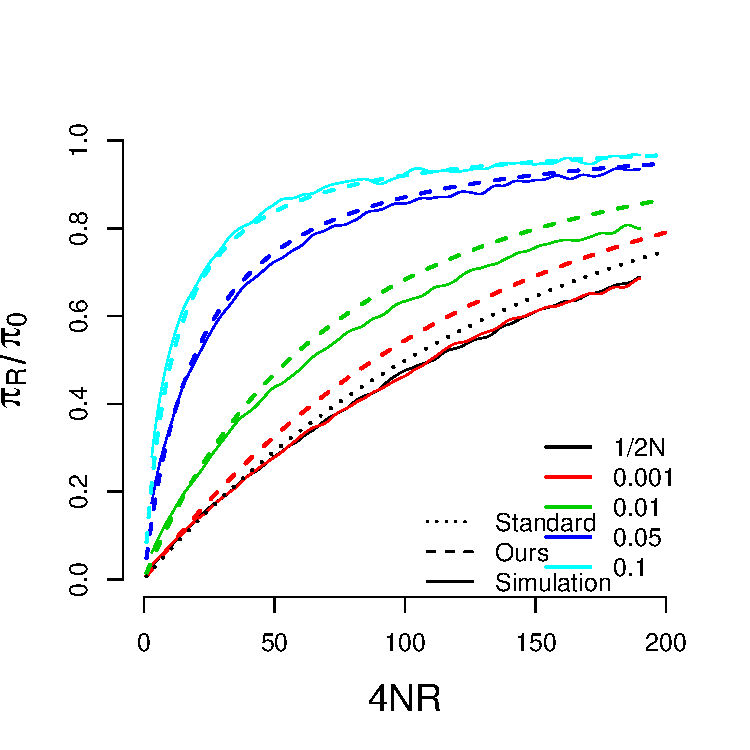
\includegraphics[width = 0.8
          \textwidth]{Paper_Figures/pi_density.pdf}
\end{figure}

\begin{figure}
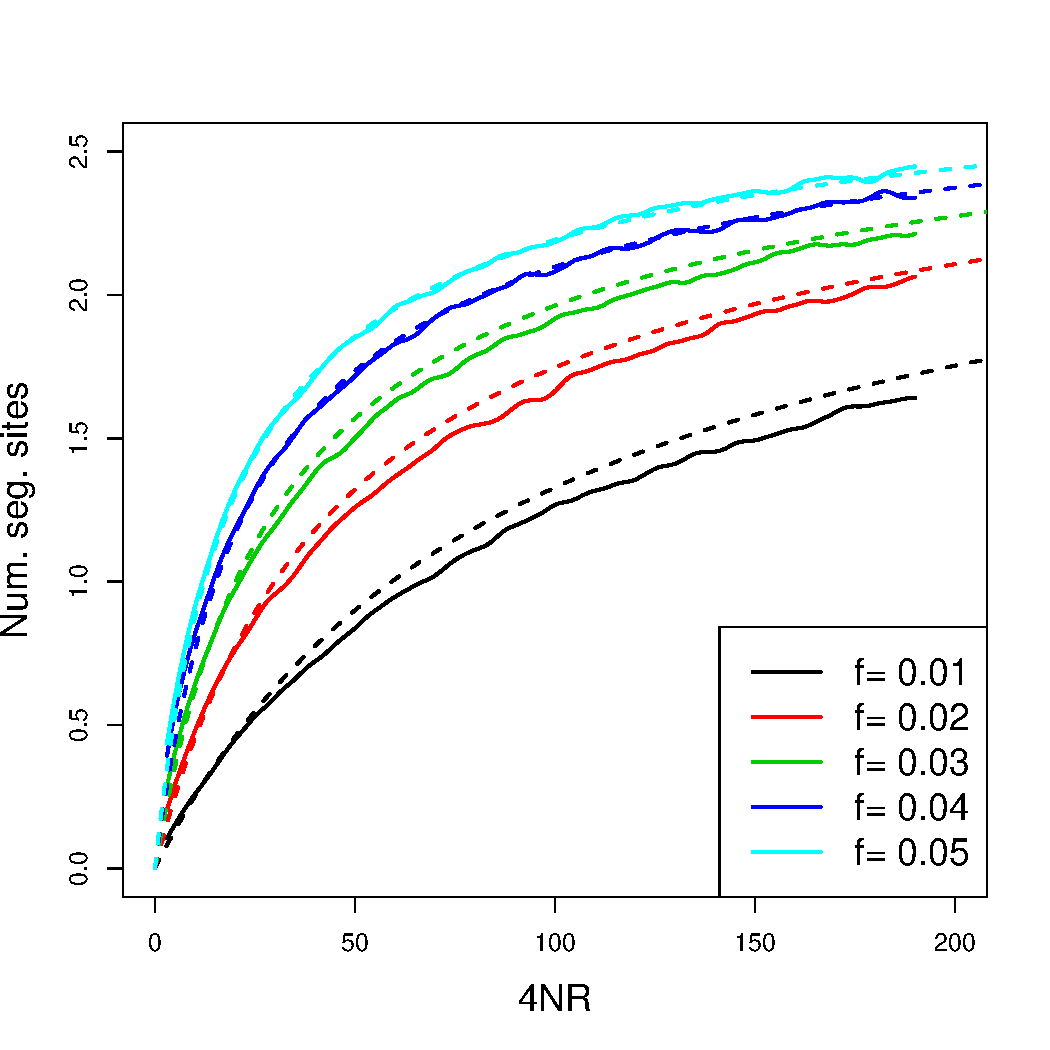
\includegraphics[width = 0.8
          \textwidth]{Paper_Figures/segsite_density.pdf}
\end{figure}

We can now reincorporate recombination during the sweep phase. Under our approximation to recombination during the sweep phase every lineage that recombines out is a singleton. So we can write the probability of having $k$ distinct lineages having recombined out of our sweep as
\begin{equation}
\sum_{i=0}^{k} {n \choose i} P_{NR}^{i} (1-P_{NR})^{n-i} p_{n-i,k-i}(R_f)
\end{equation}
as if we generate $i$ recombinant lineages during our sweep the remaining $k-i$ recombinant lineages have to come from recombination events in the neutral phase. So the expected total time in the genealogy is 
\begin{equation}
\mathbb{E}(T_{TOT})  \approx 2N \sum_{i=0}^{k} {n \choose i} P_{NR}^{i} (1-P_{NR})^{n-i} p_{n-i,k-i}(R_f)   \sum_{j=1}^{k-1} 1/j
\end{equation}
and the expected number of segregating sites can be found by taking $\mu$ times this. 

We can also obtain an expression for the frequency spectrum at sites surrounding a soft sweep. To do this we make use of a trick borrowed from \cite{Kimandstephan}, and subsequently used by \cite{NielsenKimetc}, where our frequency spectrum after a sweep reflects the fact that $k$ recombinant lineages survive through the sweep and these $k$ lineages reflect independent draws from the population frequency. This trick was also used by \citep{PenningandHermisson} to obtain the frequency spectrum of fully linked variation surrounding a soft sweep from multiple mutations, see their ``Frequency distribution of ancestral variation'' subsection in their ``Analytical Derivations'' section. We will denote the probability of sampling $j$ derived copies of a neutral allele out of a sample of $k$ by $q_{j,k}$, i.e. the neutral frequency spectrum in a sample of $k$. At a neutral site at demographic equilibrium $q_{j,k} = 1/j$ \gc{actually what do we want to do here? Do we want site to be segregating? }, otherwise it could be replaced by the empirical frequency spectrum calculated genome-wide \citep[as in ][]{NielsenKimetc}
Consider the case where no recombination occurs during the selected phase, in that case the probability of observing a neutral site segregating at a frequency of $l/n$ can be written as
\begin{equation}
p(l | n) =  \sum_{k=1}^{n}  p_{ESF}(k | R_f,n)  \sum_{j=1}^{k} q_{j,k}  p(l | k,n) 
\end{equation}
where $  p(l | k,n) $ is the probability that our $k$ recombinant lineages lead to a sample containing into $l$ derived alleles and $n-l$ alleles when the neutral allele segregates at a frequency of $j/k$ in the population before the sweep. To find this we have to sum over the possible configurations $\{a_1,\dots,a_k\}$ as follows
\begin{equation}
p(l | j, ~k,~n) = 
\sum_{\substack{a_1+\cdots a_j=l;\\
    n_{a+1}+\cdots a_k=n-l}} 
p(\{a_1,\dots,a_k\} \mid k, n) = \frac{ {n \choose l} }{ {k \choose l} }\frac{ S(l,j)  S(n-l,k-j)  }{ S(n,k) } \label{ESF_gives_freq_spec}
\end{equation}



When we allow for recombination during the sweep this expression becomes more complex, but the same logic can be followed and write
\begin{equation}
p(l | n) = \sum_{S=1}^n P_{NR}(n-S; n) \sum_{k=1}^{n-S} p_{ESF}(k | R_f,n-S) \sum_{j=1}^{S+k} q_{j,S+k}
\sum_{i=1}^{l \wedge S} B(i \mid S,j/(S+k)) p(l-i \mid j-i,k,n-S )
\end{equation}
where A$\wedge$B denotes the min(A,B). Here $S$ lineages recombine out of the selected phase, and our remaining $n-S$ lineages are partitioned into $k$ families due to recombination in the neutral phase. Out of our $S$ singleton lineages $i$ each independently choose to be of type $1$ with probability $j/(S+k)$ (i.e. binomially $ B(i \mid S,j/(S+k))$). Then in order to give rise to a sample configuration $l,~n-l$ the remaining $n-S$ lineages, who are partitioning into $k$ families, have to be paritioned into $l-i,n-S-i$ carrying 1 and 0 respectively, this happens with probability $p(l-i \mid j-i,k,n-S )$ given by eqn. \eqref{ESF_gives_freq_spec}.   

\subsubsection{Linkage Disequilibrium}
\jb{obviously needs more explication of the history of studying LD across sweeps, but will deal with later.}
\cite{StrobeckMorgan78} and \cite{Hudson85} showed that the expectation of the linkage disequilibrium statistic $D^2$ (i.e. the square of the covariance in allelic state at two loci) can be expressed as
\begin{equation}
	D^2 = F_{ij,ij} - 2F_{ij,ik} + F_{ij,kl}
\end{equation}
where the three terms are, respectively, the probability that two sequences $i$ and $j$ are identical at both sites $x$ and $y$, the probability that sequences 


\section{Discussion}


%%%%%%%%%%%%%%%%%%%%%%%%%%%%
\section{Acknowledgements}

\section{Methods}


\bibliographystyle{genetics}
\bibliography{library,morelibrary}

\section{Supplementary materials}

\setcounter{table}{0}
\renewcommand{\thetable}{S\arabic{table}}
\setcounter{figure}{0}
\renewcommand{\thefigure}{S\arabic{figure}}

\end{document}
